\documentclass{article}\usepackage[]{graphicx}\usepackage[]{color}
%% maxwidth is the original width if it is less than linewidth
%% otherwise use linewidth (to make sure the graphics do not exceed the margin)
\makeatletter
\def\maxwidth{ %
  \ifdim\Gin@nat@width>\linewidth
    \linewidth
  \else
    \Gin@nat@width
  \fi
}
\makeatother

\definecolor{fgcolor}{rgb}{0.345, 0.345, 0.345}
\newcommand{\hlnum}[1]{\textcolor[rgb]{0.686,0.059,0.569}{#1}}%
\newcommand{\hlstr}[1]{\textcolor[rgb]{0.192,0.494,0.8}{#1}}%
\newcommand{\hlcom}[1]{\textcolor[rgb]{0.678,0.584,0.686}{\textit{#1}}}%
\newcommand{\hlopt}[1]{\textcolor[rgb]{0,0,0}{#1}}%
\newcommand{\hlstd}[1]{\textcolor[rgb]{0.345,0.345,0.345}{#1}}%
\newcommand{\hlkwa}[1]{\textcolor[rgb]{0.161,0.373,0.58}{\textbf{#1}}}%
\newcommand{\hlkwb}[1]{\textcolor[rgb]{0.69,0.353,0.396}{#1}}%
\newcommand{\hlkwc}[1]{\textcolor[rgb]{0.333,0.667,0.333}{#1}}%
\newcommand{\hlkwd}[1]{\textcolor[rgb]{0.737,0.353,0.396}{\textbf{#1}}}%
\let\hlipl\hlkwb

\usepackage{framed}
\makeatletter
\newenvironment{kframe}{%
 \def\at@end@of@kframe{}%
 \ifinner\ifhmode%
  \def\at@end@of@kframe{\end{minipage}}%
  \begin{minipage}{\columnwidth}%
 \fi\fi%
 \def\FrameCommand##1{\hskip\@totalleftmargin \hskip-\fboxsep
 \colorbox{shadecolor}{##1}\hskip-\fboxsep
     % There is no \\@totalrightmargin, so:
     \hskip-\linewidth \hskip-\@totalleftmargin \hskip\columnwidth}%
 \MakeFramed {\advance\hsize-\width
   \@totalleftmargin\z@ \linewidth\hsize
   \@setminipage}}%
 {\par\unskip\endMakeFramed%
 \at@end@of@kframe}
\makeatother

\definecolor{shadecolor}{rgb}{.97, .97, .97}
\definecolor{messagecolor}{rgb}{0, 0, 0}
\definecolor{warningcolor}{rgb}{1, 0, 1}
\definecolor{errorcolor}{rgb}{1, 0, 0}
\newenvironment{knitrout}{}{} % an empty environment to be redefined in TeX

\usepackage{alltt}
\usepackage{natbib}
\usepackage[unicode=true]{hyperref}
\usepackage{geometry}
\usepackage{hyperref}
\usepackage{color}
\usepackage{amsmath}
\usepackage{amssymb}
\usepackage{verbatim}
\usepackage{mathpazo}
\usepackage{setspace}
\usepackage{multirow}
\usepackage{fullpage}
\usepackage{lscape}
\usepackage{fancyhdr}
\usepackage{wrapfig,lipsum,booktabs}
\usepackage[normalem]{ulem}
\usepackage[parfill]{parskip}
\usepackage{multirow}
\geometry{tmargin=1in,bmargin=1in,lmargin=1in,rmargin=1in}

\bibliographystyle{ecology_let}

%% for inline R code: if the inline code is not correctly parsed, you will see a message
\newcommand{\rinline}[1]{SOMETHING WRONG WITH knitr}


\IfFileExists{upquote.sty}{\usepackage{upquote}}{}
\begin{document}
\title{Workflow and detailed analyses for: "Interaction flexibility and pyrodiversity interact to increase pollinator population resistance"}
\author{Lauren Ponisio}
\maketitle

\begin{figure}[h!]
  \centering
  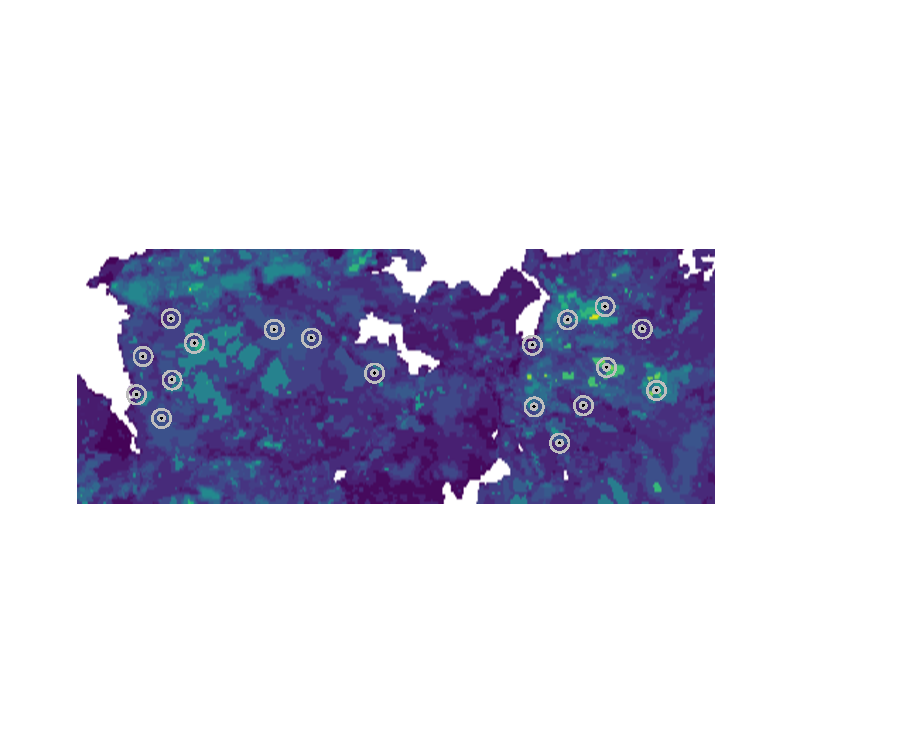
\includegraphics[width=0.9\textwidth]{figure/pyrodiv.pdf}
  \label{fig:pyrodiv}
\end{figure}
\clearpage

\section{Overview}
\label{sec:overview}

I examine the whether pyrodiversity enhances the resistance of
plant-pollinator communities and pollinator populations using a
variety of methods including 1) calculating metrics for describing
network topology 2) interaction turnover, 3) network role variability
and 4) extinction simulations. I am committed to reproducible science
and all analytical code will be maintained on github, along with this
write up.

The entire analysis is executable from the main.sh file. All of the
packages needed to run the analyses are listed in the packages.sh
file. All R scripts were run in v3.5.3. Navigate to the analysis
folder within the github repo (Yosemite) then the main.sh file can be
selected and run in terminal. This will somewhat helpfully print the
results of each analysis and re-create any accompanying figures.

I will walk through each the main script for each analysis
individually. I also outline all of the decision points for each of
the analysis.



\section{Data Prep}
\label{sec:dataprep}

In analysis/data the dataPrep.R script creates all the data structures
needed for the analyses. It references the raw data, however, so all
needed files are in the github repro and this file cannot be run.

\subsection{Decision points}
\label{sec:dataprep_dp}
\begin{enumerate}
\item Drop all non bees. Rational: non-bees not identified to species
  with the same rigor as bees. Also, life histories are less well
  understood, and bees are the more dominant pollinator in this system.
\end{enumerate}

\subsection{Pyrodiversity}
\label{sec:pyrodiv}

To estimate pyrodiversity, I developed a metric in collaboration with
Kate Wilkin to quantify the diversity of the fire histories in
relation to fire frequency, age, extent and severity experienced in an
area. This metrics was published in our previous publication
\citep{ponisio2016pyrodiversity}. We obtained fire history data of our
study area, dating back to 1984, from Yosemite National Park and the
United States Forest Service \citep{van2012factors,
miller2012Yosemite, yose2012Yosemite}.  Each fire digitization
contains rasterized values of burn severity
\citep{miller2007quantifying}.  Fire season, another component of fire
history, was not directly considered.  There was, however, little
variability in fire season within any one fire, and most fires
occurred in different months.  Thus, season is indirectly included in
the identity of each fire.

To estimate pyrodiversity, we evaluated the uniqueness of the fire
history of each raster cell $(30~\mathrm{m})^2$ resolution. We first
created categories of fire severity within a fire
\citep{miller2012Yosemite}. For each raster cell, we then used the
sequence of fires and the severity of each of those fires to define
unique fire histories.  We identified 135 unique fire histories in the
basin.  To calculate the pyrodiversity score, raster cells received
different categories if they differed in any aspect of fire history;
for example, if they were burned by the same fire but at different
severities, or if they were burned by different fires, even if at the
same severity.  Pyrodiversity was then calculated as the Simpson's
diversity of fire history categories (the compliment of the sum of the
squared proportion of each fire history category) around a monitoring
plot within $150~\mathrm{m}$.

Pragmatically, to calculate pyrodiversity, I combined the cell
values of rater layers into a single character string. I then
converted those strings to categories such that each unique fire
history experience by a cell would be a unique category.

These calculations were done for the the previous publication so the
.Rdata files are in the github repo, but not the code, specifically.

\section{Network metrics}
\label{sec:metrics}

Within the analysis/networkLevel folder, the metrics.R script runs
calculates the network topology metrics. The step to this analysis are
1) randomize the interactions within communities, 2) calculate network
metrics, 3) calculate z-scores for network metrics, 4) use linear
mixed models to estimate the relationship between pyrodiversity and
network metrics.

The analysis begins be calculating null models by constraining of a
connectance as developed by Deigo Vazquez. The algorithm was described
as follows: "The algorithm randomized the total number of individual
interactions observed in the original interaction matrix, F. To this
end, the algorithm first created a binary matrix, assigning
interspecific interactions according to species-specific
probabilities, requiring that each species had at least one
interaction. As in Vazquez et al.~(2005b), the species-specific
probabilities were proportional to species' relative abundances
(probabilities are in fact approximately proportional and not equal to
relative abundances because of the requirement that each species
receives at least one interaction; this requirement causes
probabilities to deviate from relative abundances, especially for rare
species). Once the number of filled cells in the original matrix was
reached, the remaining interactions were distributed among the filled
cells, so that connectance in the original and randomized matrices was
the same." \citep[][, page 1122-1123]{vazquez2007species}

I then used the bipartite package to calculate metrics related to
functional redundancy and complementarity. Mainly,
partner.diversity.LL" (plant Shannon's partner diversity),
"partner.diversity.HL" (pollinator Shannon's partner diversity),
"functional.complementarity.LL" (plant complementarity, based on
\citep{devoto2012understanding}), "functional.complementarity.HL"
(pollinator complementarity, based on
\citep{devoto2012understanding}), and "links.per.species" (average for
plants and for pollinators). Any metric calculated by bipartite can be
used however.

For each network metrics, I then examined the effect of pyrodiversity and drought using linear mixed models. The  equation for the models was: 
\begin{equation}
\label{equ:metrics}
\begin{aligned}
y_{i,j} & = \alpha_j + \beta1*pyrodiv_j*drought_i + \epsilon_{i,j} \\
\epsilon_{i,j} & = N(0, \sigma_{\epsilon}) \\
\alpha_j & = N(0, \sigma_{\alpha})
\end{aligned}
\end{equation}

Where $y_{i,j}$ is the network metric from the $i^{th}$ sample round
of the $j^{th}$ site, and drought is an indicator variable that is 1
in the extreme drought year and 0 otherwise. $pyrodiv_j$ is the
pyrodiversity of the $j^{th}$ site. $\alpha_i$ is the random
intercept for site.

The figures are produced by running the $plotting/networkLevel\_mods.R$ script.

\subsection{Decision points} 
\label{sec:metrics_dp}
\begin{enumerate}
\item which metrics best represent redundancy and complementarity?
  There are a plethora of metrics to chose from. I decided on the most
  direct metrics developed primarily by \citep{devoto2012understanding} for
  complementarity, and following \cite{kaiser2017ecosystem}, the partner diversity (i.e., generalization) for
  redundancy and H2 for reciprocal specialization. I considered
  nestedness as a metric of redundancy, but none of the networks were
  significantly nested.   
\end{enumerate}

\section{Community resistance}
\label{sec:comm_resist}

In the $analysis/networkLevel$ folder, the robustness.R script runs
the extinction simulations (robustness is the term for resistance to
species loss in the network world). Plants are removed sequentially
based on their abundance before the increase in drought intensity
(from lowest to highest). The pollinator species without any plant
partners left go secondarily "extinct". I modified the second.extinct
function from bipartite and then slope.bipartite to calculate the area
under the co-extinction curve \citep{Memmott2004}.

To generate the potential network, made a vector of all the plant
species a pollinator was ever observed visiting. I then filled each
network, adding a 1 in a cell if the pollinator was ever observed
visiting the corresponding plant.

The figures are produced by running the $plotting/robustness.R$ script.

  \subsection{Decision points}
  \label{sec:comm_resist_dp}
  \begin{enumerate}
  \item What order to drop plant species to simulation a drought-like
    event? Sensible options: from least to most degree or abundance
    calculated from network data or veg survey data. Veg survey data
    is based on the number of flowers vs. individuals, which is a bit
    misleading in terms of drought susceptibility. Dropping species by
    degree (sum of unique bee interaction partners at each site) and
    abundance (sum of total interactions) were qualitatively similar
    in terms on the results of the linear mixed models. Rational: drop
    species by abundance because that is the most like a drought
    perturbation (more likely to loose the least abundant first).
  \end{enumerate}

\section{Population resistance}
  \label{sec:pop_resist}

In the $analysis/variability$ folder, the steps to calculating
population resistance are as follows: 1) calculate the null
communities (again using vaznull) in order to standardize partner
"$\beta$-diversity" (nulls.R), 2) calculate partner turnover
(partner.R), 3) calculate role variability (pca.R), then 4) the change
in abundance of each pollinator species at each site (deltaAbund.R)
and then the linear mixed models. To test whether the variability
metrics were indeed an accurate representation of variability, I
generated communities with no to high variability and examined the
values of the variability scores ($test_flex_mets.R$). The variability
metrics for partners and roles were small when the interaction
matrices generated had little interaction turnover, and high with high
interaction turnover, as intended.

Dissimilarity estimates can be affected by the total number of
species/interactions sampled at a site \citep[e.g.,][]{Chase2011}. So
I used null models to estimate the deviation of the observed
$\beta$-diversity from that which would be expected under a random
community assembly process, with constrained connectance and
approximately constrained marginals.  I then calculated the fraction
of randomly assembled communities with dissimilarity values less than
(and half of those equal to) that of the observed community. I used
this fraction as a ``corrected dissimilarity score'' for our observed
data.  Corrected dissimilarity values near one indicate that the
observed communities exhibit more species turnover between sites than
expected under a random assembly process while values near $0.5$
indicate that the observed communities exhibit levels of turnover more
in line with the null expectation.

The general equation for the models was: 
\begin{equation}
  \label{equ:pop_resist}
\begin{aligned}
y_{i,j} & = \alpha_i + \beta_1*pyrodiv_j*partnerVar_i +
\beta_2*pyrodiv_j*roleVar_i + \\
& \beta_3*meanRole_i + 
beta_4*deltaFlowers_j + \epsilon_{i,j} \\
\epsilon_{i,j} & = N(0, \sigma_{\epsilon}) \\
\alpha_j & = N(0, \sigma_{\alpha})
\end{aligned}
\end{equation}

Where $y_{i,j}$ is the log ratio abundance from the $i^{th}$ species
at the $j^{th}$ site. $pyrodiv_j$ is the pyrodiversity of the $j^{th}$
site, $partnerVar_i$ is the partner variability of the $i^{th}$
species, $roleVar_i$ is the network role variability of the $i^{th}$
species, $meanRole_i$ is the average network role (mean PCA1 score) of
the $i^{th}$ species, and $deltaFlowers_j$ is the change in floral
richness of the $j^{th}$ between the years $2013$ (drought) and $2014$
(extreme drought).  $\alpha_i$ is the random intercept for pollinator
species.


\subsection{Decision points}
  \label{sec:pop_resist_dp1}
\subsubsection{Partner turnover}
\begin{enumerate}
\item Null models: Constrain alpha diversity and not the number of
  individuals in the null models for calculating the expected
  $\beta$-diversity. Rational: Little difference in the results when
  different null models are used \citep{ponisio2015farm}
\item Turnover calculation: weight interactions by their ``abundance''
  vs. binary interactions and use Chao as a dissimilarity
  estimate. Rational: turnover in the number of interactions is
  ecological meaningful and a part of interaction flexibility. Chao
  \citep{Chao2005} is density invariant, replication invariance, and
  monotonic.
\item Turnover calculation: calculate the corrected interaction
  turnover by using the Chase et al. (calculating the fraction of
  randomly assembled communities with dissimilarity values less than
  and half of those equal to that of the observed
  community). Rational: calculating the corrected turnover using
  z-scores (the alternative) was not qualitatively different
  \citep{ponisio2015farm}.
\item Species-specific turnover calculation: the CV of the turnover
  across all sampling periods (both through time at a site and across
  sites) in 2013. Rational: 2013 is our baseline, pre-extreme drought
  data point. Interaction flexibility can be both within a season (at
  the same site through time and different plant come into and out of
  bloom) and across sites (re-shuffle the plant community
  composition). Other options, 1) cv corrected by samples size, an
  unbiased estimates when sample sizes are low. Ruled out because
  sample size is not particularly small. The pvalue
  for the interaction between partner variability and pyrodiversity
  becomes marginal (0.06), but this does not substantially change the
  results (unless you are very militant about pvalues). 2) sd. Ruled
  out because does not control for mean. 
\end{enumerate}

\subsubsection{Role turnover}
  \label{sec:pop_resist_dp2}
\begin{enumerate}
\item Role quantification: chose "rarefied degree",
  "weighted.betweenness", "weighted.closeness", "niche.overlap",
  "species.strength", "d" as representatives of a species network
  role. Rational: These metrics cover a range different aspects of a
  species' role, though there is some overlap. Choose different
  similar metrics did not change results qualitatively.
\item Role variability calculation: CV of pca1 scores for each species
  across samples in 2013. Rational: CV measures the variability while
  controlling for the mean of values. SD and corrected CV rules out
  for same reasons as with partner variability. pca1 is the primary
  axis for differentiating roles. Interaction flexibility can be both
  within a season (at the same site through time and different plant
  come into and out of bloom) and across sites (re-shuffle the plant
  community composition).
\end{enumerate}
  
\subsubsection{Linear mixed models}
  \label{sec:pop_resist_dp3}
\begin{enumerate}
  \item drop two species with really extreme values of role
    flexibility. Rational: from examining their interactions, they
    seem to have occupied basically the exact same role in every
    network they were observed in (though interestingly different
    species). The model diagnostic look a lot better without including
    them. In addition, the model results are mostly
    consistent. Removing them makes the coefficient for pyrodiversity
    less negative, as expected by removing an extreme value that is
    shaping the slope. 
  \end{enumerate}


\section{Resource availability}
  \label{sec:resource}
For the supplemental information, I made figures for the change in
  flower richness between the yers 2013 and 2014. These analyses were
  included in \cite{ponisio2016pyrodiversity}.


\clearpage
\bibliography{network}
\clearpage


\end{document}
